\section{Results}

\subsection{Path Shape}
\FloatBarrier
\begin{figure}[!htb]
\begin{minipage}{0.33\textwidth}
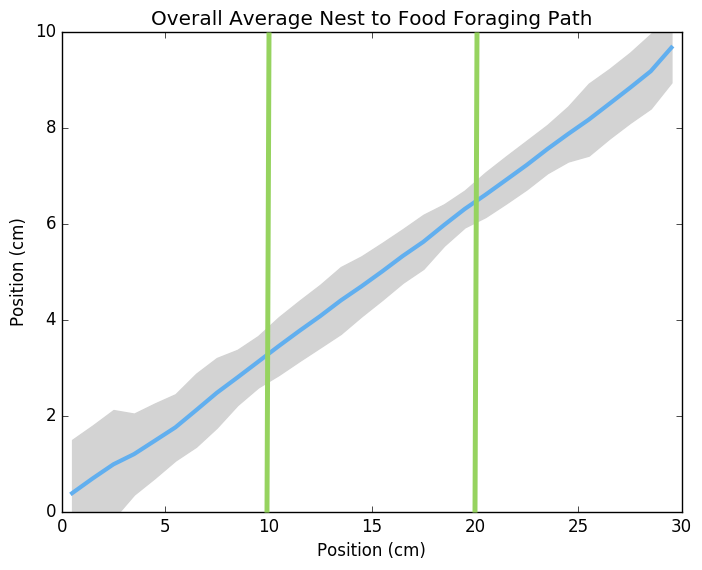
\includegraphics[width=\textwidth]{img/corner-to-corner-average_path_negpidiv3.png}
\end{minipage}%
\begin{minipage}{0.05\textwidth}
\end{minipage}%
\begin{minipage}{0.33\textwidth}
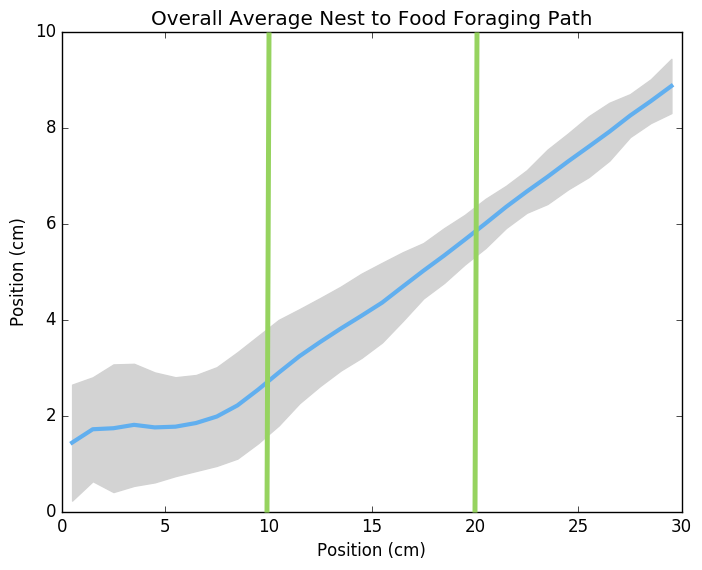
\includegraphics[width=\textwidth]{img/corner-to-corner-average_path_0.png}
\end{minipage}%
\begin{minipage}{0.05\textwidth}
\end{minipage}%
\begin{minipage}{0.33\textwidth}
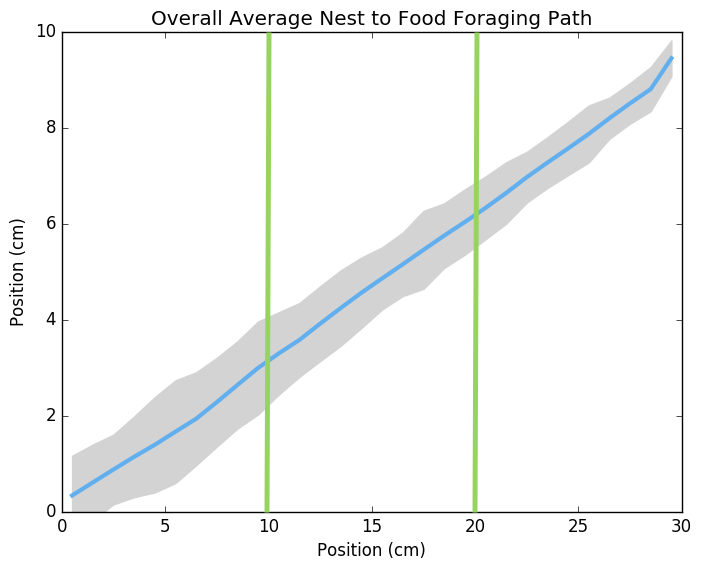
\includegraphics[width=\textwidth]{img/corner-to-corner-average_path_pidiv3.png}
\end{minipage}%

\caption{Comparison of overall average nest to food foraging path for, left to right, $-\pi/3$, $0$, and $\pi/3$ radian inclines.}
\end{figure}


\subsection{Path Length}
\FloatBarrier
\begin{figure}[!htb]
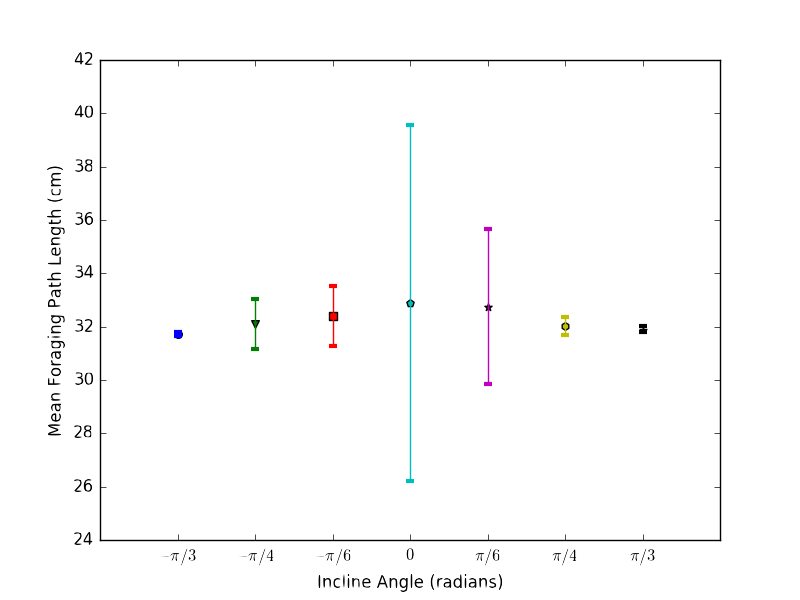
\includegraphics[width=0.4\textwidth]{img/corner-to-cornermeanforagingpathlength.png}
\caption{Comparison of path lengths over incline angles for corner-to-corner trials}
\end{figure}


\subsection{Trip Duration}
\FloatBarrier
\begin{figure}[!htb]
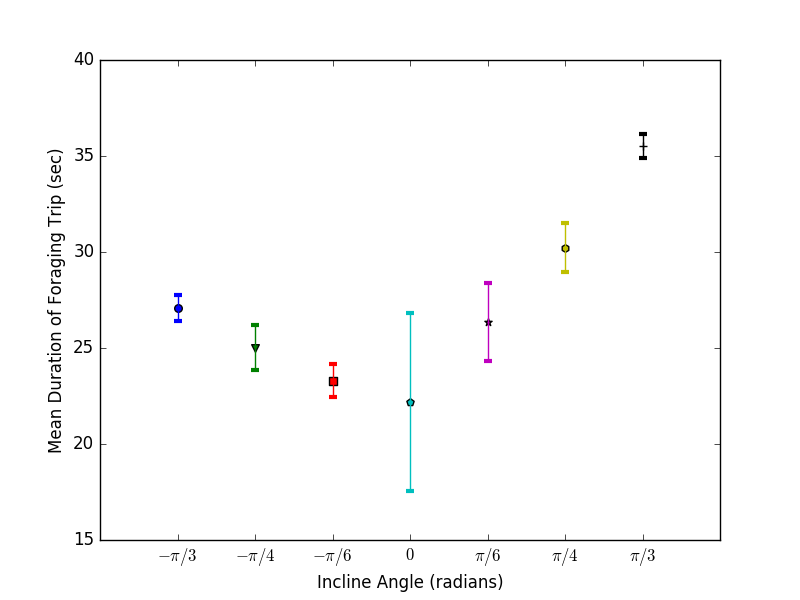
\includegraphics[width=0.4\textwidth]{img/corner-to-cornermeandurationofforagingtrip.png}
\caption{Comparison of trip durations over incline angles for corner-to-corner trials}
\end{figure}


\subsection{Summary}
\begin{itemize}
	\item as expected, foraging trips take longer over steeper incline and decline
	\begin{itemize}
		\item also taking longer over uphill versus downhill inclines
	\end{itemize}
	\vspace{1em}

	\item the foraging path is generally more stable with steep incline or decline
	\begin{itemize}
		%\item path is smoother
		\item ants are less likely to get lost/stuck
		\item this effect is less pronounced in the center-to-center arena
	\end{itemize}
	\vspace{1em}

	\item the foraging path becomes more direct with steeper incline or decline
	\vspace{-1em}
	\begin{itemize}
		\item even though the direct path is not aligned with the incline in the corner-to-corner arena
		\item this effect is less pronounced in the center-to-center arena
	\end{itemize}
\end{itemize}
